%----------------------------------------------------------------------------------------
%	PACKAGES AND THEMES
%----------------------------------------------------------------------------------------
\documentclass[aspectratio=169,xcolor=dvipsnames]{beamer}
\usetheme{SimplePlus}
\setbeamertemplate{footline}[frame number]{}

\usepackage{hyperref}
\usepackage{graphicx} % Allows including images
\usepackage{booktabs} % Allows the use of \toprule, \midrule and \bottomrule in tables
\usepackage{siunitx}
\usepackage{import}
\usepackage{amsmath}
%\numberwithin{equation}{section}% numera eq come #section.#formula
\usepackage{amsthm}
\usepackage{stmaryrd}
\usepackage{amssymb}
\usepackage{wasysym}
\usepackage{cancel}
\usepackage{textcomp}
\usepackage{subcaption}
\definecolor{myred}{rgb}{0.545, 0.172, 0.031}
%\usepackage{cleveref}
%----------------------------------------------------------------------------------------
%	TITLE PAGE
%----------------------------------------------------------------------------------------

\title[short title]{Risposta strutturale di elementi strutturali laminati} % The short title appears at the bottom of every slide, the full title is only on the title page
\subtitle{Laminato composito CF/PEEK ad uso biomedicale}

\author[Pin-Yen] {Alessandro Mastrofini}

\institute[NTU] % Your institution as it will appear on the bottom of every slide, may be shorthand to save space
{
Meccanica Computazionale dei Tessuti e Biomateriali \\
Università degli Studi di Roma Tor Vergata% Your institution for the title page
}
\date{2022} % Date, can be changed to a custom date

\graphicspath{{figures/}} %Setting the graphicspat%h
\graphicspath{{figures/}} %Setting the graphicspath
\makeatletter
\providecommand*{\input@path}{}
\edef\input@path{{figures/}{}\input@path}% prepend
\makeatother
%----------------------------------------------------------------------------------------
%	PRESENTATION SLIDES
%----------------------------------------------------------------------------------------

\begin{document}

\begin{frame}
    % Print the title page as the first slide
    \titlepage
\end{frame}

%------------------------------------------------
\section{First Section}
%------------------------------------------------

\begin{frame}{Composite laminate}
    \begin{figure}%[b!]  %% Add a [b!] if you prefer the wide image to be at the bottm of the page
    	  \centering
    	  	\begin{minipage}{\linewidth}
    	  		\centering
  	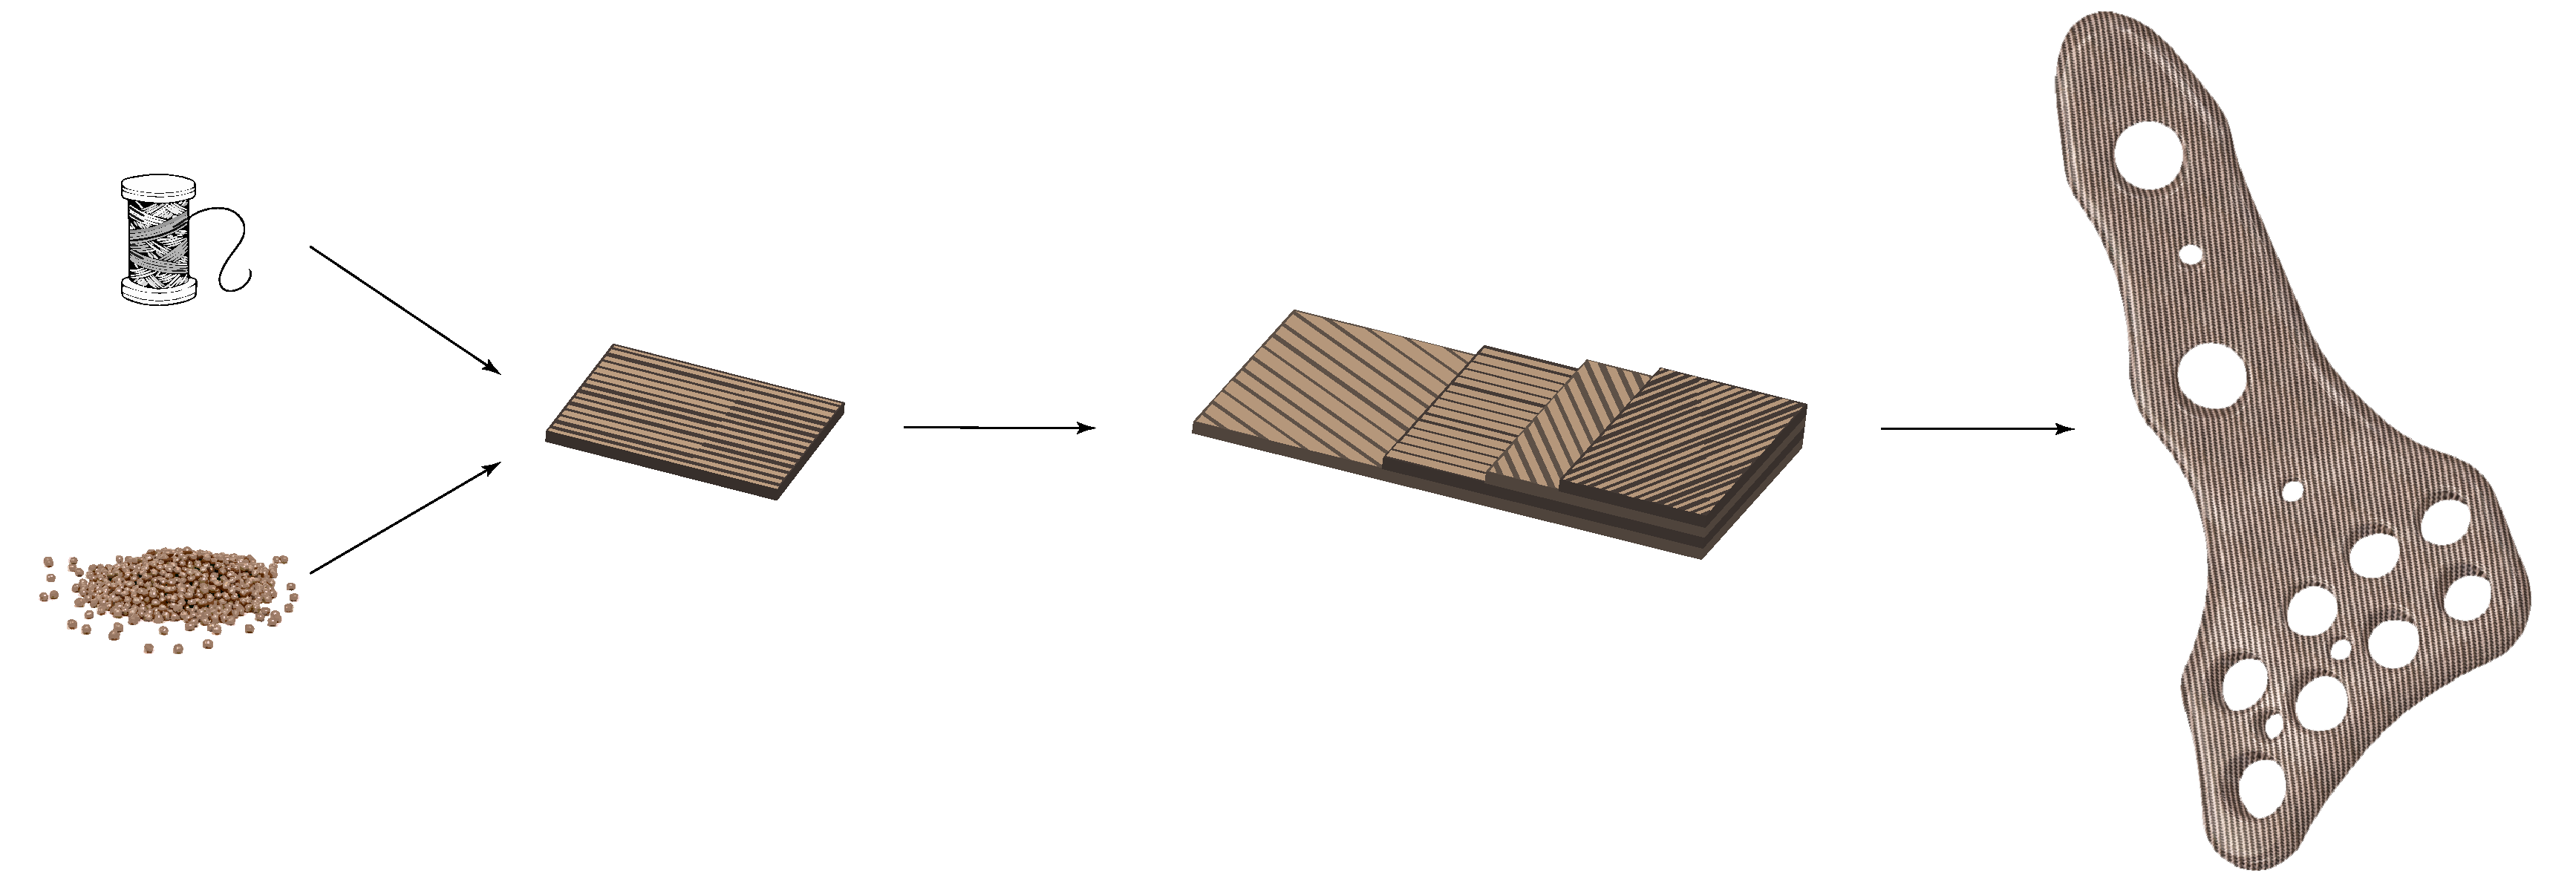
\includegraphics[width=0.9\textwidth]{laminate_figures.pdf}
\end{minipage}
\pause
  				\begin{minipage}{0.5\linewidth}
  					\centering
  		\begin{figure}\scalebox{0.5}{
  				\def\svgwidth{1.3\linewidth}
  				\input{miture_rule_result_tex.pdf_tex}}
  		\end{figure}
  	\end{minipage}
			\scalebox{0.55}{\begin{minipage}{0.3\linewidth}
			\begin{equation*}
v_{m}+f_{f}=1
			\end{equation*}				
		\begin{equation*}
E_{1}=f_{f} E_{f}+\left(1-f_{f}\right) E_{m}
		\end{equation*}				
		\begin{equation*}
		E_{2}=\left(\frac{1-f_{f}}{E_{m}}+\frac{f_{f}}{E_{f}}\right)^{-1}
	\end{equation*}
	\begin{equation*}
G_{12}=\left(\frac{v_{m}}{G_{m}}+\frac{v_{f}}{G_{f}}\right)^{-1}
	\end{equation*}
		\end{minipage}}\hspace{50pt}
	\end{figure}
\end{frame}
%%
%
%
\begin{frame}{Layout}
	
\begin{figure}

\begin{minipage}{0.35\textwidth}
	
	\begin{minipage}{0.45\textwidth}
	\tiny{	\def\svgwidth{\linewidth}
		\input{struct1_tex.pdf_tex}}
	\end{minipage}\hfill
	\begin{minipage}{0.45\textwidth}
		\tiny{	\def\svgwidth{\textwidth}
		\input{struct2_tex.pdf_tex}}
	\end{minipage}\hfill
	\begin{minipage}{0.45\textwidth}
		\tiny{	\def\svgwidth{\textwidth}
		\input{struct3_tex.pdf_tex}}
	\end{minipage}\hfill
	\begin{minipage}{0.45\textwidth}
		\tiny{	\def\svgwidth{\textwidth}
		\input{struct4_tex.pdf_tex}}
	\end{minipage}\hfill
\end{minipage}\hspace{0.07\linewidth}
%%%%%%%%%%%%%
\begin{minipage}{0.55\textwidth}
	\begin{minipage}{0.45\textwidth}
			\centering
	\scalebox{0.5}{	\def\svgwidth{2\linewidth}
	\input{plate_tex.pdf_tex}}
	\end{minipage}\hfill
	\begin{minipage}{0.45\textwidth}
		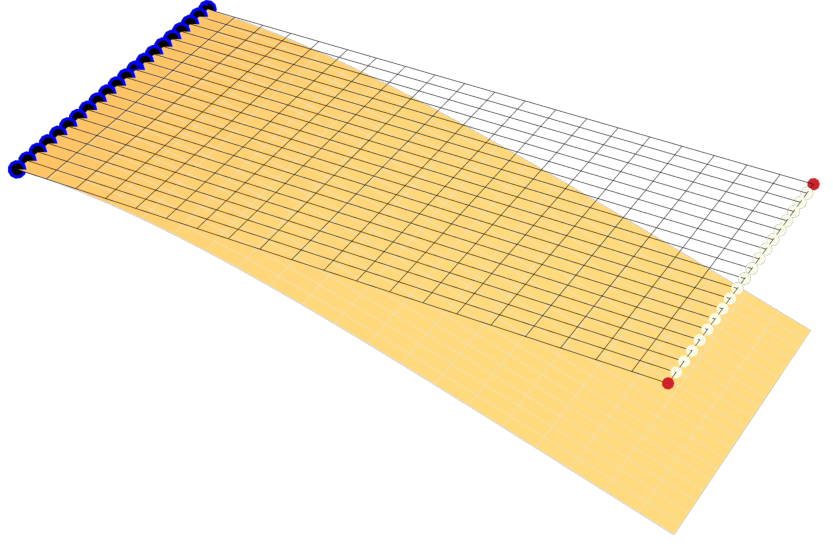
\includegraphics[width=\textwidth]{/first_test/alpha=40.pdf}
	\end{minipage}\hfill
	\begin{minipage}{0.45\textwidth}
	\scalebox{0.5}{	\def\svgwidth{2\linewidth}
\input{cyl_tex.pdf_tex}}
	\end{minipage}\hfill
	\begin{minipage}{0.45\textwidth}
		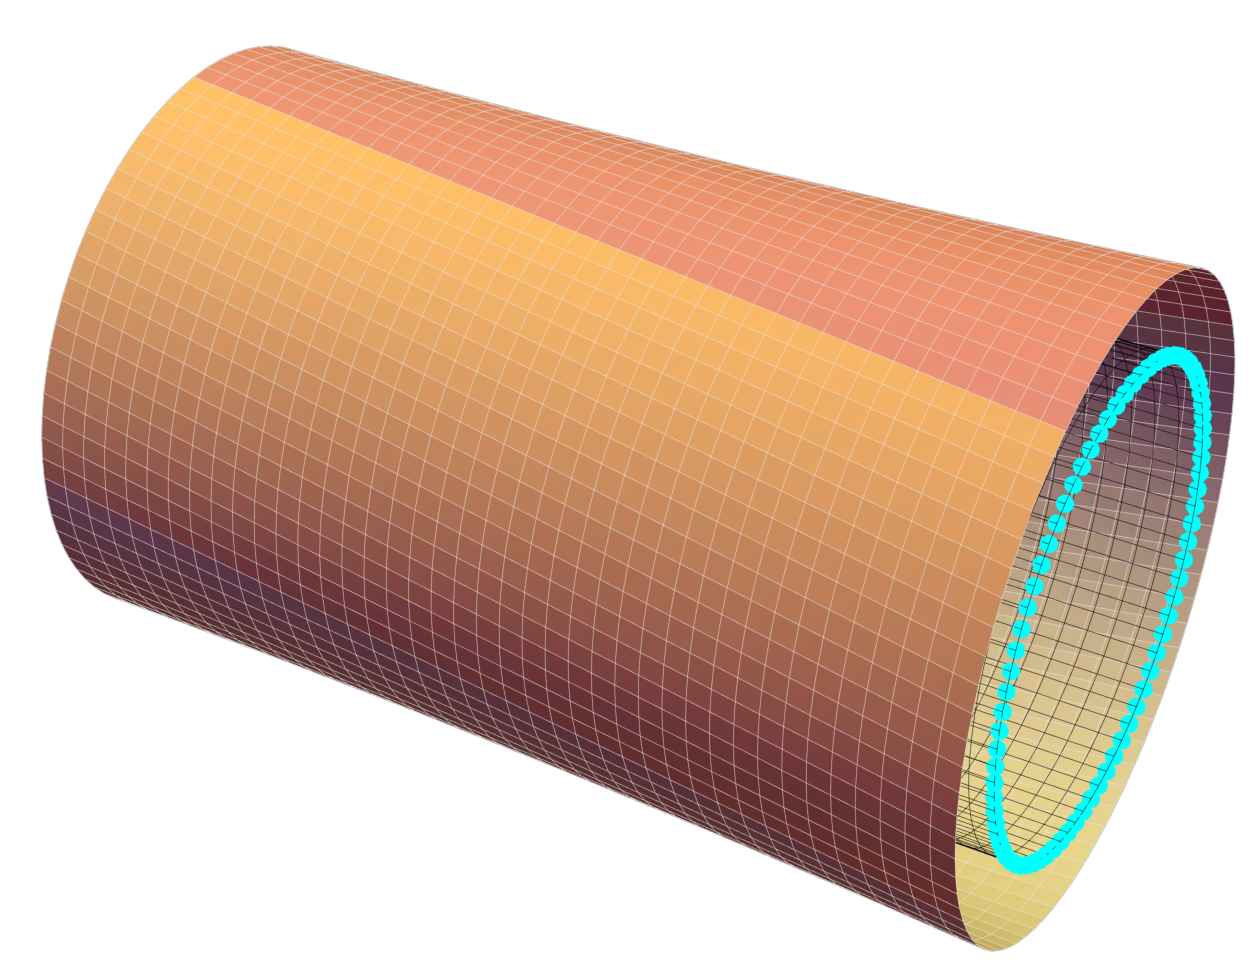
\includegraphics[width=\textwidth]{/more_test/cyl_30_45_30_45.pdf}
	\end{minipage}
\end{minipage}\hfill

\end{figure}
\end{frame}

\begin{frame}{Parametric analysis}
\begin{figure}
	\centering
	
	\begin{minipage}{\linewidth}
			\centering
	\begin{minipage}{0.3\textwidth}
		\centering
		\scalebox{.5}{
		\tiny{	\def\svgwidth{2\linewidth}
			\input{first_test_bothload_V_X.pdf_tex}}}

		
	\end{minipage}
	\hfill
	\begin{minipage}{0.3\textwidth}
		\centering
		\scalebox{.5}{
				\tiny{	\def\svgwidth{2\linewidth}
			\input{first_test_bothload_W_Y.pdf_tex}}}
		
		
	\end{minipage}
	\hfill
	\begin{minipage}{0.3\textwidth}
		\centering
		\scalebox{.5}{
				\tiny{	\def\svgwidth{2\linewidth}
			\input{first_test_bothload_W_X.pdf_tex}}}

		
	\end{minipage}	\hfill

\end{minipage}
	\begin{minipage}{\linewidth}
	\centering
	
	\begin{minipage}{0.3\textwidth}
		\centering
		\scalebox{.5}{
				\tiny{	\def\svgwidth{2\linewidth}
			\input{first_test_transload_V_X.pdf_tex}}}

		
	\end{minipage}
	\hfill
	\begin{minipage}{0.3\textwidth}
		\centering
		\scalebox{.5}{
				\tiny{	\def\svgwidth{2\linewidth}
			\input{first_test_transload_W_Y.pdf_tex}}}
		

		
	\end{minipage}
	\hfill
	\begin{minipage}{0.3\textwidth}
		\centering
		\scalebox{.5}{
				\tiny{	\def\svgwidth{2\linewidth}
			\input{first_test_transload_W_X.pdf_tex}}}

	\end{minipage}	\hfill
	\end{minipage}
	\begin{minipage}{\linewidth}
	\centering
	
	\begin{minipage}{0.3\textwidth}
		\centering
		\scalebox{.5}{
				\tiny{	\def\svgwidth{2\linewidth}
			\input{first_test_axialload_V_X.pdf_tex}}}

		
	\end{minipage}
	\hfill
	\begin{minipage}{0.3\textwidth}
		\centering
		\scalebox{.5}{
				\tiny{	\def\svgwidth{2\linewidth}
			\input{first_test_axialload_W_Y.pdf_tex}}}
		

		
	\end{minipage}
	\hfill
	\begin{minipage}{0.3\textwidth}
		\centering
		\scalebox{.5}{
			\tiny{		\def\svgwidth{2\linewidth}
			\input{first_test_axialload_W_X.pdf_tex}}}

	\end{minipage}	\hfill
	\end{minipage}

\end{figure}

\end{frame}


\begin{frame}{Layout analysis}
\begin{figure}
	\centering
	%%%%%%%%%%%%%%%%%%%%%%%%%%%%%%%%%%%%%%
	\begin{minipage}{\linewidth}
		\hspace{0.05\linewidth}
	\begin{minipage}{0.1\textwidth}
\tiny{	\def\svgwidth{\textwidth}
	\input{struct3_tex.pdf_tex}}
\end{minipage}\hfill
		\begin{minipage}{0.18\textwidth}
			\centering
			\scalebox{.5}{
				\tiny{	\def\svgwidth{2\linewidth}
					\input{fabric_bothload_V_X.pdf_tex}}}
		\end{minipage}
		\hfill
		\begin{minipage}{0.18\textwidth}
			\centering
			\scalebox{.5}{
				\tiny{	\def\svgwidth{2\linewidth}
					\input{fabric_bothload_W_Y.pdf_tex}}}
		\end{minipage}
		\hfill
		\begin{minipage}{0.18\textwidth}
			\centering
			\scalebox{.5}{
				\tiny{	\def\svgwidth{2\linewidth}
					\input{fabric_bothload_W_X.pdf_tex}}}
		\end{minipage}	\hfill
	\end{minipage}\vspace{5pt}
%%%%%%%%%%%%%%%%%%%%%%%%%%%%%%%%%%%%%%%%%%%%%%%%%%%
	\begin{minipage}{\linewidth}
	\centering
	\begin{minipage}{0.2\textwidth}
		\centering
		\scalebox{.5}{
			\tiny{	\def\svgwidth{2\linewidth}
				\input{deformata_D_tex.pdf_tex}}}
	\end{minipage}
	\hfill
		\begin{minipage}{0.24\textwidth}
		\centering
		\scalebox{.5}{
			\tiny{	\def\svgwidth{2\linewidth}
				\input{BD_bothload_V_X.pdf_tex}}}
	\end{minipage}
	\hfill
	\begin{minipage}{0.24\textwidth}
		\centering
		\scalebox{.5}{
			\tiny{	\def\svgwidth{2\linewidth}
				\input{BD_bothload_W_Y.pdf_tex}}}
	\end{minipage}
	\hfill
	\begin{minipage}{0.24\textwidth}
		\centering
		\scalebox{.5}{
			\tiny{	\def\svgwidth{2\linewidth}
				\input{BD_bothload_W_X.pdf_tex}}}
	\end{minipage}	\hfill
\end{minipage}\vspace{10pt}
%%%%%%%%%%%%%%%%%%%%%%%%%%%%%%%%%%
\begin{minipage}{\linewidth}
\begin{minipage}{0.2\textwidth}
	\centering
	\scalebox{.5}{
		\tiny{	\def\svgwidth{2\linewidth}
			\input{first_test_C_V_X.pdf_tex}}}
\end{minipage}\hfill
	\begin{minipage}{0.2\textwidth}
		\centering
		\scalebox{.5}{
			\tiny{	\def\svgwidth{2\linewidth}
				\input{first_test_C_V_X_2.pdf_tex}}}
	\end{minipage}\hfill
		\begin{minipage}{0.2\textwidth}
			\centering
			\scalebox{.5}{
				\tiny{	\def\svgwidth{2\linewidth}
					\input{first_test_C_W_X.pdf_tex}}}
		\end{minipage}\hfill
				\begin{minipage}{0.2\textwidth}
				\centering
				\scalebox{.5}{
					\tiny{	\def\svgwidth{2\linewidth}
						\input{first_test_C_W_X_2.pdf_tex}}}
			\end{minipage}\hfill
\end{minipage}
%%%%%%%%%%%%%%%%%%%%%%%%%%%%%%%%%%
\begin{minipage}{\linewidth}
	
	\begin{minipage}{0.2\textwidth}
		\centering
		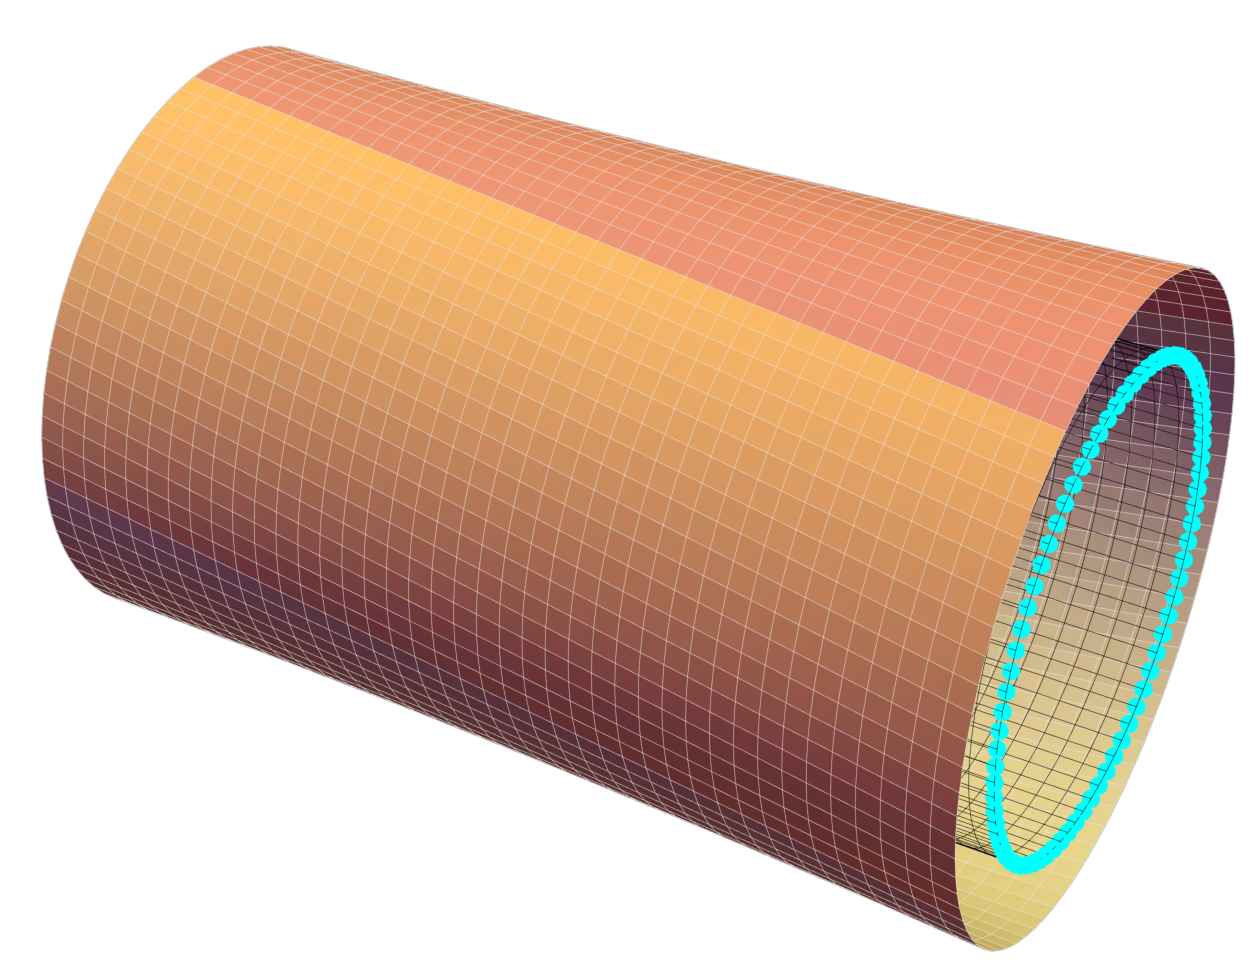
\includegraphics[width=\textwidth]{/more_test/cyl_30_45_30_45.pdf}
	\end{minipage}\hfill
	\begin{minipage}{0.2\textwidth}
		\centering
		\scalebox{.5}{
			\tiny{	\def\svgwidth{2\linewidth}
				\input{D_extra_tex.pdf_tex}}}
	\end{minipage}\hfill
	\begin{minipage}{0.2\textwidth}
		\centering
		\scalebox{.5}{
			\tiny{	\def\svgwidth{2\linewidth}
				\input{BD_C_V_X.pdf_tex}}}
	\end{minipage}\hfill
	\begin{minipage}{0.2\textwidth}
		\centering
		\scalebox{.5}{
			\tiny{	\def\svgwidth{2\linewidth}
				\input{BD_C_W_X.pdf_tex}}}
	\end{minipage}\hfill
\end{minipage}


	\end{figure}

\end{frame}

\begin{frame}{Plate thickness}
\begin{figure}

%%%%%%%%%%%%%%%%%%%%%%%%%%%%%%%%%%
\begin{minipage}{\linewidth}
	\hspace{0.1\linewidth}
	\begin{minipage}{0.1\textwidth}
		\centering
	\scalebox{.5}{
	\tiny{	\def\svgwidth{2\linewidth}
		\input{struct5_tex.pdf_tex}}}
	\end{minipage}\hfill
	\begin{minipage}{0.12\textwidth}
		\centering
		\scalebox{.5}{
			\tiny{	\def\svgwidth{2\linewidth}
				\input{struct5_thickness.pdf_tex}}}
	\end{minipage}\hfill
	\begin{minipage}{0.15\textwidth}
		\centering
		\scalebox{.5}{
			\tiny{	\def\svgwidth{2\linewidth}
				\input{struct5_thickness_sigmaX_.pdf_tex}}}
	\end{minipage}	\hspace{0.1\linewidth}\hfill
\end{minipage}

%%%%%%%%%%%%%%%%%%%%%%%%%%%%%%%%%%
\begin{minipage}{\linewidth}
	\begin{minipage}{0.3\textwidth}
		\centering
		\scalebox{.5}{
			\tiny{	\def\svgwidth{2\linewidth}
				\input{last_layer_V_X.pdf_tex}}}
	\end{minipage}\hfill
	\begin{minipage}{0.3\textwidth}
		\centering
		\scalebox{.5}{
			\tiny{	\def\svgwidth{2\linewidth}
				\input{last_layer_W_Y.pdf_tex}}}
	\end{minipage}\hfill
	\begin{minipage}{0.3\textwidth}
		\centering
		\scalebox{.5}{
			\tiny{	\def\svgwidth{2\linewidth}
				\input{last_layer_W_X.pdf_tex}}}
	\end{minipage}\hfill
\end{minipage}

%%%%%%%%%%%%%%%%%%%%%%%%%%%%%%%%%%
\begin{minipage}{\linewidth}
	\begin{minipage}{0.3\textwidth}
		\centering
		\scalebox{.5}{
			\tiny{	\def\svgwidth{2\linewidth}
				\input{grafico_sigma_x.pdf_tex}}}
	\end{minipage}\hfill
	\begin{minipage}{0.3\textwidth}
		\centering
		\scalebox{.5}{
			\tiny{	\def\svgwidth{2\linewidth}
				\input{grafico_sigma_y.pdf_tex}}}
	\end{minipage}\hfill
	\begin{minipage}{0.3\textwidth}
		\centering
		\scalebox{.5}{
			\tiny{	\def\svgwidth{2\linewidth}
				\input{grafico_tau_xy.pdf_tex}}}
	\end{minipage}\hfill
\end{minipage}

\end{figure}

\end{frame}

\end{document}